\documentclass[12pt,a4paper]{report}

\usepackage{geometry}
\geometry{left=25mm, right=25mm, top=25mm, bottom=25mm}
\usepackage{setspace}
\setstretch{1.5}
\usepackage{titlesec}
\usepackage{tocloft}
\usepackage{graphicx}
\usepackage{amsmath}
\usepackage{caption}
\usepackage{enumitem}
\usepackage{float}
\usepackage{booktabs}
\usepackage{hyperref}
\usepackage{comment}
\usepackage{natbib}
\usepackage{subcaption}
\usepackage{tikz}
\usetikzlibrary{shapes.geometric}

\title{Automation of nuclear material cladding coating measurement process }
\author{Emma Tekulová }

\titleformat{\chapter}[hang]{\bfseries\LARGE}{\thechapter.}{1em}{}
\titleformat{\section}[hang]{\bfseries\Large}{\thesection}{1em}{}
\titleformat{\subsection}[hang]{\bfseries\large}{\thesubsection}{1em}{}
\titleformat{\subsubsection}[hang]{\bfseries\normalsize}{\thesubsubsection}{1em}{}


\renewcommand{\cftchapfont}{\bfseries}
\renewcommand{\cftsecfont}{\normalfont}
\renewcommand{\cftchappagefont}{\bfseries}
\renewcommand{\cftsecleader}{\cftdotfill{\cftdotsep}}


\usepackage{titlesec}

\usepackage{titlesec}

\titleformat{\chapter}[display]
  {\normalfont\huge\bfseries} 
  {}{0pt}{} 
  \titlespacing*{\chapter}{0pt}{-1cm}{\baselineskip} % Adjust vertical space before the chapter title


\begin{document}

\maketitle
\newpage


\chapter*{Summary}
The data used in this work are from researchers using scanning electron microscope images to investigate the properties of oxidation and coating layers on various materials essential to the nuclear industry. Accurately measuring the thickness of these layers is important for material characterization. The current manual measurement process is time-consuming, and automating it can significantly improve efficiency. Many algorithms can assist with automation, varying widely in complexity and input expectations. While many of these algorithms promise powerful and accurate results, real-world scenarios require substantial groundwork before these tools can be effectively deployed and automation established. This work discusses the challenges and solutions encountered, beginning with the collection and assessment of all available data. It then explores experiments with both conventional computer vision and machine learning algorithms, evaluating their performance. The overall parameters of different solutions are examined, and the most suitable approach is selected. This approach is then seamlessly integrated into the researchers' existing workflow.
\newpage
\chapter*{Souhrn}
Data použitá v této práci pocházejí od výzkumníků, kteří využívají snímky ze skenovacího elektronového mikroskopu ke zkoumání vlastností oxidačních a povlakových vrstev na různých materiálech důležitých pro jaderný průmysl. Přesné měření tloušťky těchto vrstev je klíčové pro charakterizaci materiálů. Současný manuální proces měření je časově náročný a jeho automatizace může výrazně zvýšit efektivitu. Existuje mnoho algoritmů, které mohou pomoci s automatizací, přičemž se liší svojí složitostí a požadavky na vstupní data. Ačkoli mnoho z nich nabízí přesné a výkonné výsledky, v realitě si jejich nasazení vyžaduje rozsáhlou přípravu, aby bylo možné efektivně dosáhnout automatizace. Tato práce se zabývá výzvami a řešeními, které byly při vývoji automatizovaného řešení identifikovány. Začíná sběrem a analýzou dostupných dat, následně se věnuje experimentům s konvenčními algoritmy počítačového vidění a strojového učení, přičemž hodnotí jejich výkonnost. Jsou zhodnoceny parametry různých řešení a vybraný nejvhodnější přístup, který je následně integrován do stávajícího pracovního postupu.
\newpage



\chapter*{Acknowledgements}

    
I would like to express my gratitude to my advisor, \textbf{Ing. Petr Čech, Ph.D.}, and my consultant, \textbf{Mgr. Jaroslav Knotek}, for their guidance and support throughout this work.
\\
The input data used was created with state support from the Technology Agency of the Czech Republic under the THÉTA Program as part of project No. TK04030082 and utilizing the CICRR infrastructure, which is financially supported by the Ministry of Education, Youth, and Sports – project LM2023041.

\newpage

\renewcommand{\contentsname}{\vspace{-1.5cm}Contents}
\addtocontents{toc}{\vspace{-1cm}}
\tableofcontents


\newpage


\chapter{Introduction}

The Research Institute Řež conducts numerous projects within the nuclear industry, many of which involve electron microscopy and the analysis of materials exposed to high temperatures and aggressive environments, such as those found in nuclear reactors. A significant portion of these projects requires extensive manual image analysis, making automation a key challenge. Currently, image analysis is performed using various processing tools, including Fiji~\cite{Schindelin2012} by ImageJ. This thesis aims to automate one of these manual processes.

The images analyzed in this thesis are part of a project that includes two main image categories: material samples with protective coating layers and samples with extensive oxidation and no coating. This work focuses exclusively on the coated samples, which typically exhibit more uniform and structured features compared to the irregular and heterogeneous appearance of the oxidized samples. Examples of both image types are shown in Figure~\ref{fig:coating-oxidation}. The coated images originate from a study investigating the thickness and integrity of cladding layers applied to various materials, both before and after exposure to high temperatures and aggressive environments, with the aim of evaluating their protective performance. This thesis focuses on the automated measurement of the coating layers. Although the current work is limited to coated samples, the methods developed here may later be adapted for use with the more complex oxidized samples.


To address the segmentation task, three computer vision approaches are explored, ranging from traditional clustering methods to advanced deep learning models. The first method investigated is K-means clustering, an unsupervised algorithm that does not require labeled data. Although K-means offers a lightweight and accessible approach, its performance is constrained by the complex and non-homogeneous nature of the coating layers. Variability in layer structure, color, and visual features requires image-specific parameter tuning, which limits its general usability. A more detailed evaluation of this method is presented in Section~\ref{sec:kmeans}.



\begin{figure}[H]
    \centering
    \begin{subfigure}{0.4\textwidth}
        \centering
        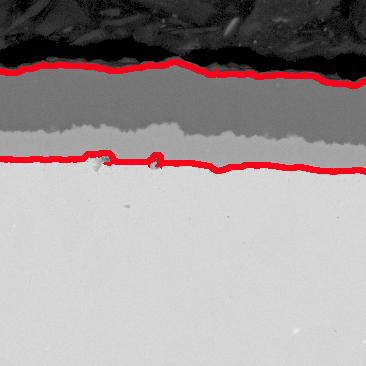
\includegraphics[width=\linewidth]{PICTURES/intro/177_CROP.png}
        \caption{Cropped image showing a protective coating layer highlighted in red.}         
        \label{fig:coating}
    \end{subfigure}
    \hfill
    \begin{subfigure}{0.4\textwidth}
        \centering
        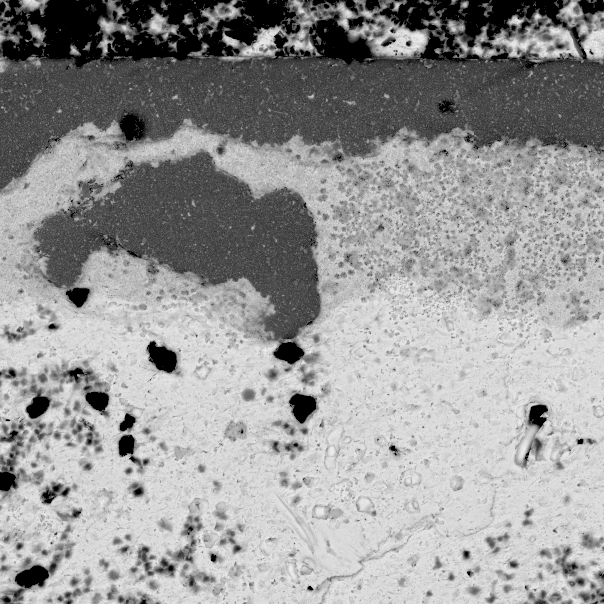
\includegraphics[width=\linewidth]{PICTURES/intro/625_3500h_low_cross_strana1_13_crop.png}
     \caption{Cropped image of a sample exhibiting oxidation without coating.} \label{fig:oxidation}        
     \label{fig:oxidation}
    \end{subfigure}
    \caption{Examples of coating and oxidation layers in material samples.}
    \label{fig:coating-oxidation}
\end{figure}


The second method involves the Segment Anything Model (SAM)\cite{kirillov2023segany}, a state-of-the-art segmentation approach based on transformers. SAM is designed for general-purpose segmentation and demonstrates considerable potential due to its flexibility and robust architecture. However, it requires significantly higher computational resources and, in practice, was found to lack the specificity and precision needed for accurate segmentation of coating and oxidation layers. This limitation is further analyzed in Section~\ref{sec:sam}.

The third approach utilizes Convolutional Neural Networks (CNNs), which demand labeled training data but are capable of achieving high segmentation accuracy once trained. In this work, three types of labels were developed for training and evaluation. Initially, no ground truth annotations were available. To address this, the Fiji image processing software—commonly used by scientists for manual analysis—was modified to support manual annotation while capturing precise measurement data. This enhancement enabled the creation of the first type of labels: polygon-based annotations.

During the manual annotation process, the results from a previous experiment using K-means clustering were collected to generate a second dataset. However, K-means struggled to reliably distinguish between coating and oxidation, especially in more complex cases. To address this, a third label type, called refined K-means, was introduced. These labels were manually adjusted versions of the K-means labels, corrected and improved using image editing tools by researchers. This final set of labels represents the most accurate annotations and serves as the ground truth for evaluating the CNN models. A more detailed discussion on the CNN approach and label development is provided in Section~\ref{sec:cnn}.

Following the creation of the label sets, a CNN model was developed and trained using the refined K-means annotations. The model underwent hyperparameter tuning to optimize its performance. For comparison, additional models were trained on the first and second label types to estimate their expected performance in future applications.

The final model was evaluated not only on a dedicated test dataset but also in a practical setting by researchers. This evaluation considered both segmentation accuracy and the time required for image analysis, as discussed in Sections~\ref{sec:res} and~\ref{sec:resprec}. Given the limited size of the initial dataset, the long-term goal is to establish a feedback loop: by automating the labeling process, more samples can be efficiently annotated. This expanded dataset would, in turn, allow the model to further improve its performance, continuously enhancing both the speed and accuracy of the image analysis workflow.

This thesis is structured as follows: Sections~\ref{sec:kmeans} and~\ref{sec:sam} discuss the two image segmentation methods and why they could not be implemented. Section~\ref{sec:cnn} discusses label creation and model training based on the CNN approach. Section~\ref{sec:integ} describes the integration of the trained model into the existing labeling software. The results, including analysis of segmentation accuracy and time efficiency, are presented in Sections~\ref{sec:res} and~\ref{sec:resprec}. Finally, Section~\ref{chap:con} concludes the thesis with a summary and a discussion of potential future developments.


\chapter{Practical Part}
\section{Data}

The dataset consists of images captured using a scanning electron microscope (SEM). These images are part of a study focused on the thickness of coating cladding layers applied to various materials, both before and after being subjected to high temperatures and aggressive environments, to assess the properties of these layers. The layers of interest are marked within red rectangular boxes in Figure~\ref{fig:three-images}. These layers exhibit varied characteristics, such as differences in color, number of layers, and degrees of damage.

\begin{figure}[ht]
    \centering
    \begin{subfigure}{0.3\textwidth}
        \centering
        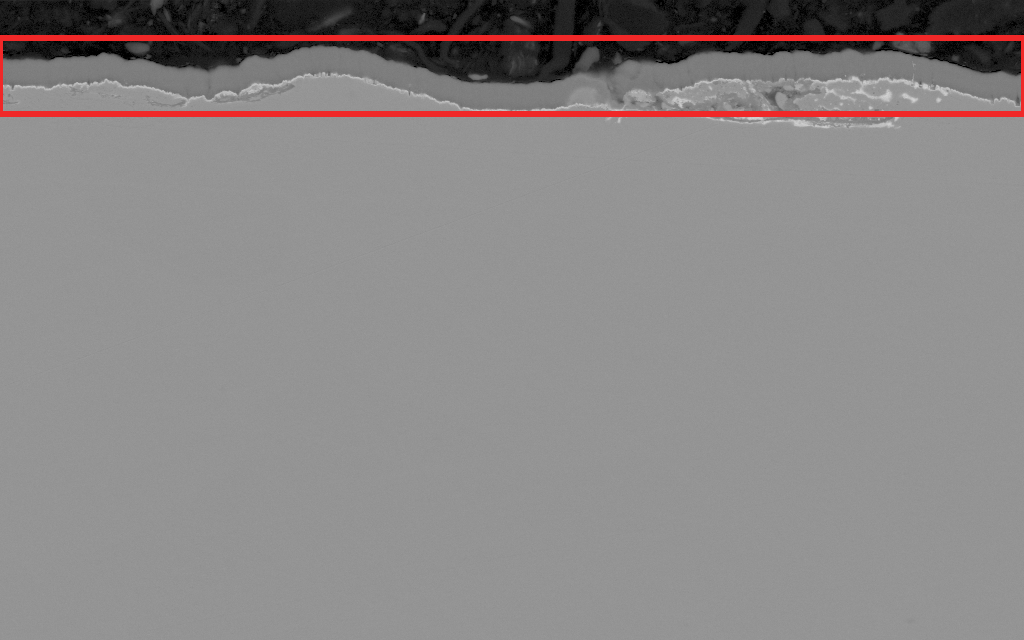
\includegraphics[width=\linewidth]{PICTURES/original_data/11.png}
        \label{fig:subfig1}
    \end{subfigure}
    \hfill
    \begin{subfigure}{0.3\textwidth}
        \centering
        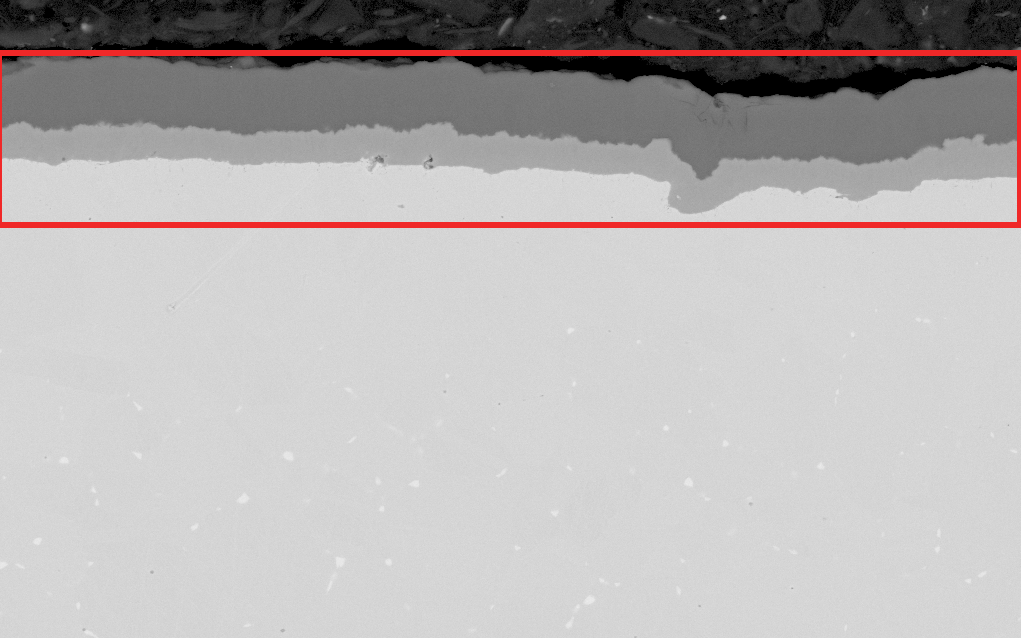
\includegraphics[width=\linewidth]{PICTURES/original_data/177.png}
        \label{fig:subfig2}
    \end{subfigure}
    \hfill
    \begin{subfigure}{0.3\textwidth}
        \centering
        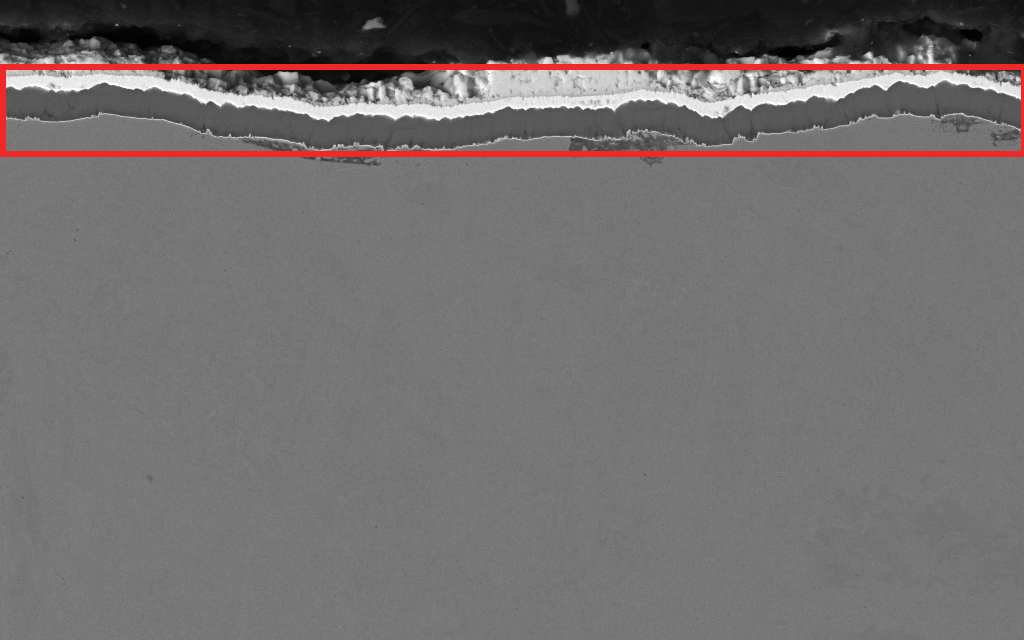
\includegraphics[width=\linewidth]{PICTURES/original_data/208.png}
        \label{fig:subfig3}
    \end{subfigure}
    \caption{SEM images with highlighted coating layers in red boxes.}
    \label{fig:three-images}
\end{figure}

\subsection{Manual Data Processing}\label{sec:ManualProc}

The images are initially obtained in *.tif format after the measurements with the SEM. Then they are processed using Fiji, an open-source image processing software that is a distribution of ImageJ \cite{Schindelin2012}. A predefined template consisting of 20 lines is used for measurements, each corresponding to a specific measurement region. The first ten lines, indexed 1 to 10, are employed to measure the thickness of the coating layer, while the second set of ten lines, located beneath the first, are used to measure oxidation. The lines are evenly distributed across the image's width and share a constant x-coordinate.

Subsequent to the initial measurements, each of the 20 lines is manually adjusted to align with either the oxidation or the coating layer. After all adjustments are completed, the measurements are exported to Excel for statistical analysis. If a layer is absent at the location of a predefined line, the line is left in its position but is later marked as 0.0 in the corresponding Excel spreadsheet. 

The images are grouped into batches of approximately 30, with each batch containing images of the same material, though different parts of the material are captured in each image, leading to a high degree of similarity among the images in each batch. The initial image of each batch typically takes longer to process since the line adjustments from the previous image are reused for the other images in the same batch. As the remaining images within a batch are more similar, they require less time for adjustment. The primary challenges arise in images where significant oxidation is present, which may destroy the coating layer.

Figure~\ref{fig:Fiji} illustrates the measurements performed in Fiji. Lines 1 to 10, used for measuring the coating layer, are shown. In this example, no oxidation layer is present.

\begin{figure}[H]
    \centering
    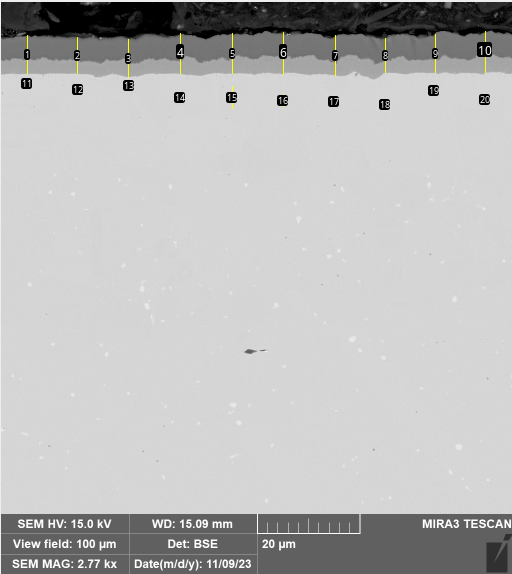
\includegraphics[width=0.7\linewidth]{PICTURES/625_Al2O3_3500h_low_cross_strana2_13_measurements.png}
    \caption{Measurement in Fiji software.}
    \label{fig:Fiji}
\end{figure}

\newpage
Although oxidation and coating layers are both critical for material characterization, this thesis focuses specifically on automating the measurement of coating layer thickness in SEM images. Coating layers prevent underlying materials from oxidizing, making oxidation layers less common in samples that feature coatings.


\subsection{Fiji Adjustments}\label{sec:1.2.2}

The first modification involved the customization of the `StartUpMacro` in Fiji, which runs automatically each time the program is launched. Three new buttons were incorporated into the interface: one for saving measurements, another for adjusting the scale, and a third for displaying the default lines.

The \texttt{Save Measurement} button was implemented to store data from the 20 lines required to create the dataset necessary for automation. This feature ensures that the required measurements are automatically saved.

The \texttt{Adjust Scale} button was added to streamline user interaction with Fiji, addressing the need to manually adjust the scale at the start of each session. Since the scale, visible at the bottom of the image, remains constant across all images, this functionality simplifies the process.

The \texttt{Set Default ROI} button was introduced to allow the researcher to quickly access the prepared default 20 lines for new batch.

Furthermore, the extraction of the final measured lengths into an Excel file was simplified.

\subsection{Dataset}

As previously mentioned, the first step in dataset creation was gathering data. Prior to this, results were stored exclusively in Excel tables, which included the lengths of the measurement lines but lacked positional information, rendering them insufficient for generating a comprehensive dataset. After collecting enough data thanks to the Fiji adjustments~\ref{sec:1.2.2}, stored in a zip folder containing 20 *.roi files (each representing one measurement line), the dataset was created.

\subsubsection{Polygon Labels}

The initial set of labels was generated using measured data from ten measurement lines. The upper ten points of each line were connected to form a boundary curve, and the same process was applied to the lower points. The space between these two curves was then filled to generate the mask. However, due to missing information at the edges of the image, cropping of both the images and the masks was needed. Figures~\ref{fig:polygon_sem_color} and~\ref{fig:polygon_sem} illustrate that the masks do not extend to the edges of the images.

This labeling process was automated using a Python script. The script loads each image along with the corresponding zip folder containing the line measurements. The x and y coordinates of these lines are stored in arrays, which are then mapped onto an Excel sheet. Any lines marked as missing (labeled as 0) in Excel are excluded, even if they are present in the folder.

To interpolate the boundary points, cubic spline interpolation \cite{fritsch1980monotone} was employed. The upper and lower boundary points, stored in arrays, were used to create a spline model, which was then applied to generate the boundary curve. The interpolation function was used with a smoothing parameter of s=0 to ensure that the interpolation closely followed the measured points. The space between the curves was filled, resulting in a binary mask. The mask was resized to match the original image dimensions and saved as a binary mask.

This approach enabled the automated generation of masks from the measured oxidation lines, ensuring that the labels were consistent with the scientific data.



\subsubsection{K-means Labels} \label{sec:kmeans}

The K-means algorithm \cite{lloyd1982least} is a clustering method used in unsupervised machine learning, designed to minimize a function that measures the quality of cluster formation. The algorithm selects $k$ random points as cluster centers from the dataset, assigning each data point to the nearest center based on distance. The geometric center of each cluster is then recalculated, and the process repeats until a convergence criterion is met.

K-means is particularly effective for images with distinct pixel colors. One of the key advantages of K-means is that it does not require prior labels, but the value of $k$ (the number of clusters) must be chosen carefully. Thus, the optimal $k$ was determined through testing for each batch of images.

In most cases, further processing was necessary, particularly to isolate the coating layer while eliminating noise. As illustrated in Figures~\ref{fig:kmean_sem_color} and~\ref{fig:kmean_sem}, K-means encountered difficulty distinguishing between oxidation and the coating layer, as their pixel values were similar and even formed a continuous cluster. Consequently, the algorithm alone was insufficient for accurately measuring the coating layer.

\subsubsection{K-means Refined}

To improve the accuracy of the K-means labels, the entire dataset was reviewed collaboratively with the researcher, and the masks were manually refined using image editing software. These manually refined masks, considered the most accurate, were validated by the researcher. The final version of the masks was then used as a test dataset for further automation.


\begin{figure}[ht]
    \centering
    \begin{subfigure}{0.3\textwidth}
        \centering
        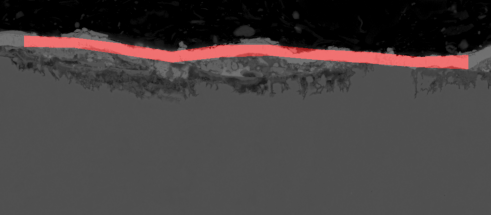
\includegraphics[width=\linewidth]{PICTURES/MASK/POLYGON316L_W_3500h_low_cross_strana1_07.png}
        \caption{Polygon mask}
        \label{fig:polygon_sem_color}
    \end{subfigure}
    \hfill
    \begin{subfigure}{0.3\textwidth}
        \centering
        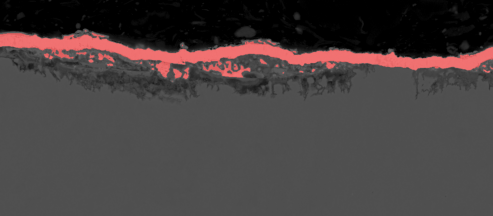
\includegraphics[width=\linewidth]{PICTURES/MASK/KMEAN316L_W_3500h_low_cross_strana1_07.png}
        \caption{K-Means mask}
        \label{fig:kmean_sem_color}
    \end{subfigure}
    \hfill
    \begin{subfigure}{0.3\textwidth}
        \centering
        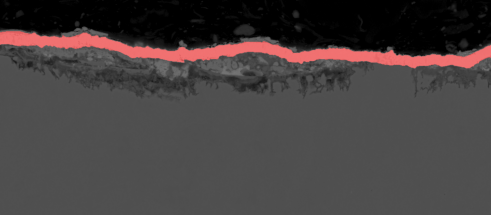
\includegraphics[width=\linewidth]{PICTURES/MASK/149_original.png}
        \caption{Refined K-Means}
        \label{fig:kmean_refined_color}
    \end{subfigure}
    \caption{Masks on SEM image}
    \label{fig:three-masks_color}
\end{figure}

\begin{figure}[ht]
    \centering
    \begin{subfigure}{0.3\textwidth}
        \centering
        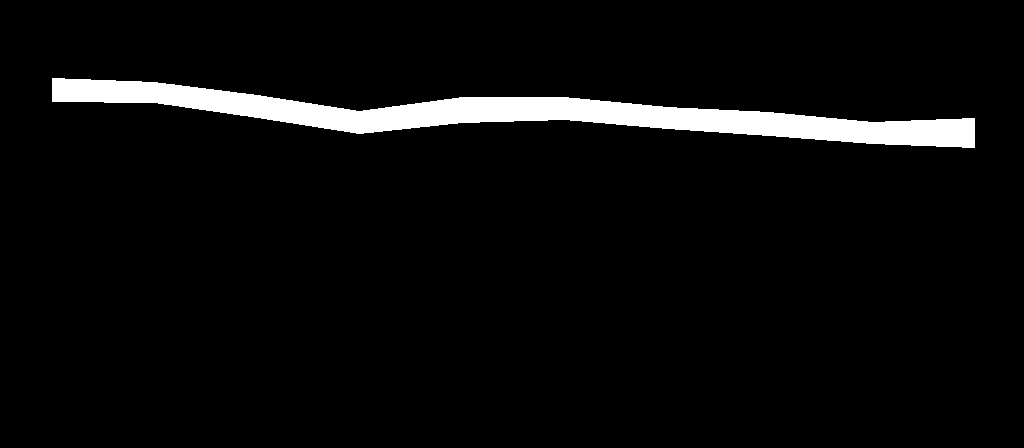
\includegraphics[width=\linewidth]{PICTURES/MASK/316L_W_3500h_low_cross_strana1_07(2).png}
        \caption{Polygon mask}
        \label{fig:polygon_sem}
    \end{subfigure}
    \hfill
    \begin{subfigure}{0.3\textwidth}
        \centering
        
\includegraphics[width=\linewidth]{PICTURES/MASK/316L_W_3500h_low_cross_strana1_07.png}
        \caption{K-Means mask}
        \label{fig:kmean_sem}
    \end{subfigure}
    \hfill
    \begin{subfigure}{0.3\textwidth}
        \centering
        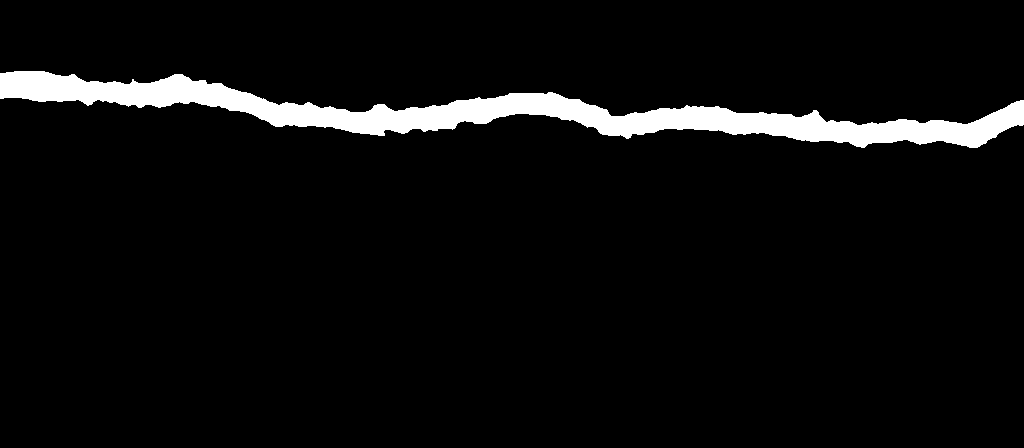
\includegraphics[width=\linewidth]{PICTURES/MASK/316L_W_3500h_low_cross_strana1_07(1).png}
        \caption{Refined K-Means}
        \label{fig:kmean_refined_sem}
    \end{subfigure}
    \caption{Binary masks}
    \label{fig:three-masks}
\end{figure}


\newpage
\section{Convolutional Neural Networks}\label{sec:cnn}

As discussed in the previous section, K-Means clustering struggled to distinguish between the oxidation and coating layers in complex samples. Additionally, K-Means has the limitation of requiring a fixed set of hyperparameters and postprocessing strategies, which cannot be generalized across different batches of images. This makes it unsuitable for automating the measurement process. In contrast, Convolutional Neural Networks (CNNs)\cite{oshea_introduction_2015} offer a promising solution to these challenges . CNNs are supervised machine learning models, well-suited for tasks involving spatial hierarchies in images, where the relationship between pixels and their positions is crucial.

For this task, the U-Net architecture\cite{ronneberger2015unetconvolutionalnetworksbiomedical} is particularly effective. U-Net has shown strong performance in various segmentation problems, especially in biomedical imaging. Unlike typical CNNs used for classification, U-Net is designed for pixel-wise classification, making it ideal for tasks requiring precise localization of objects, such as in microscopy images.

\subsection{U-Net Architecture}

The U-Net architecture consists of two main components:

\begin{itemize}
    \item \textbf{Contracting path (Encoder)}: The left side of the U-Net includes a series of convolutional, activation, and pooling layers that progressively reduce the image's dimensions. This part extracts features from the input image.
    
    \item \textbf{Expanding path (Decoder)}: The right side of the U-Net gradually upsamples the feature maps back to the original image size. This step recovers spatial resolution lost during downsampling and ensures precise pixel-wise segmentation.
\end{itemize}

\begin{figure}[H]
    \centering
    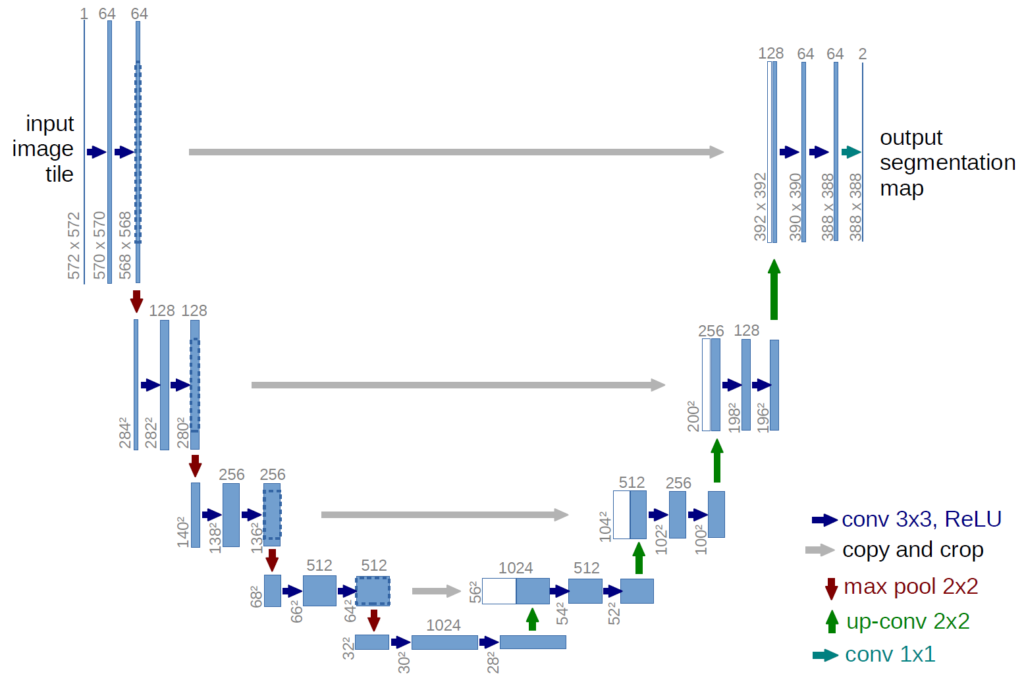
\includegraphics[width=0.8\linewidth]{PICTURES/unet-architecture.png}
    \caption{U-Net architecture \cite{ronneberger_u-net_2015}}
    \label{fig:unet-architecture}
\end{figure}

The input to a U-Net model is typically an image of size $H \times W \times C$, where $H$ is the height, $W$ is the width, and $C$ is the number of input channels. In Figure~\ref{fig:unet-architecture}, the input consists of grayscale images, where $C = 1$. For RGB images, $C = 3$. The output is an image of size $H \times W \times N$, where $N$ is the number of segmentation classes. In this case, there are two classes (binary segmentation), so $N = 2$.

\subsubsection{Upsampling with Transpose Convolutions}

The expanding path uses transpose convolutions (also called deconvolutions). Convolution reduces the image to a feature map, while transpose convolution upsamples the feature map back into an image.

\subsubsection{Skip Connections}

During the downsampling process, the network learns various features. However, as the feature maps shrink, details are lost. Skip connections allow the network to preserve these details by carrying them over from the earlier layers in the contracting path to the corresponding layers in the expanding path. This process helps retain important spatial information, improving segmentation accuracy. These connections are represented by the horizontal arrows in Figure~\ref{fig:unet-architecture}.
\subsubsection{Key Steps in U-Net Processing}
\begin{enumerate}
    \item In the contracting path, feature maps are progressively downsampled until the lowest resolution is reached.
    \item Before each downsampling step, feature maps are saved.
    \item During the upsampling process, saved feature maps are combined with the upsampled maps to recover spatial details \cite{ronneberger_u-net_2015}.
\end{enumerate}

\subsection{U-net and Microscopy}
A 2023 survey \cite{wu_state---art_2024} highlights U-Net as an effective model for microscopic image segmentation. This success is attributed to its ability to perform well with limited training data and its relatively quick training process. The survey also emphasizes the use of the original, unmodified U-Net, which has been widely applied in fields such as cytology and geology \cite{chen_deep_2020} (e.g., using scanning electron microscopy). Given that the images in this dataset share similar characteristics, the U-Net architecture is considered suitable for this task.

\subsection{Data Preprocessing – Augmentation}
The dataset consists of 150 training images, which are divided into training and validation subsets, along with 47 test images. To enhance the model's ability to generalize to unseen data, data augmentation is applied to train data.

The first step involves cropping the images to a predefined $n \times n$ size, where $n$ represents the patch size, a model hyperparameter. Cropping is done using the \textit{CropNonEmptyMaskIfExists}\cite{info11020125} function. This function ensures that the cropped region always contains parts of the coating, preserving important features. The cropping is applied with a probability of $p=1.0$, ensuring its occurrence.

Additional augmentations are applied with a probability of $p=0.3$ to increase variability. These include:

\begin{itemize}
    \item \textbf{Brightness and contrast adjustment:}This simulates lighting variations.
    \item \textbf{Sharpening:} This enhances the details in the image.
    \item \textbf{Horizontal flipping:} The image is mirrored along the horizontal axis to reduce positional bias.
    \item \textbf{Elastic transformation:} A non-linear deformation is applied to simulate distortions and improve generalization. It is applied with a probability of $p=0.5$.
\end{itemize}

The effects of these augmentations are illustrated in Figure \ref{fig:augmentation}, where different transformations are applied to a sample image.

\begin{figure}[H]
\centering
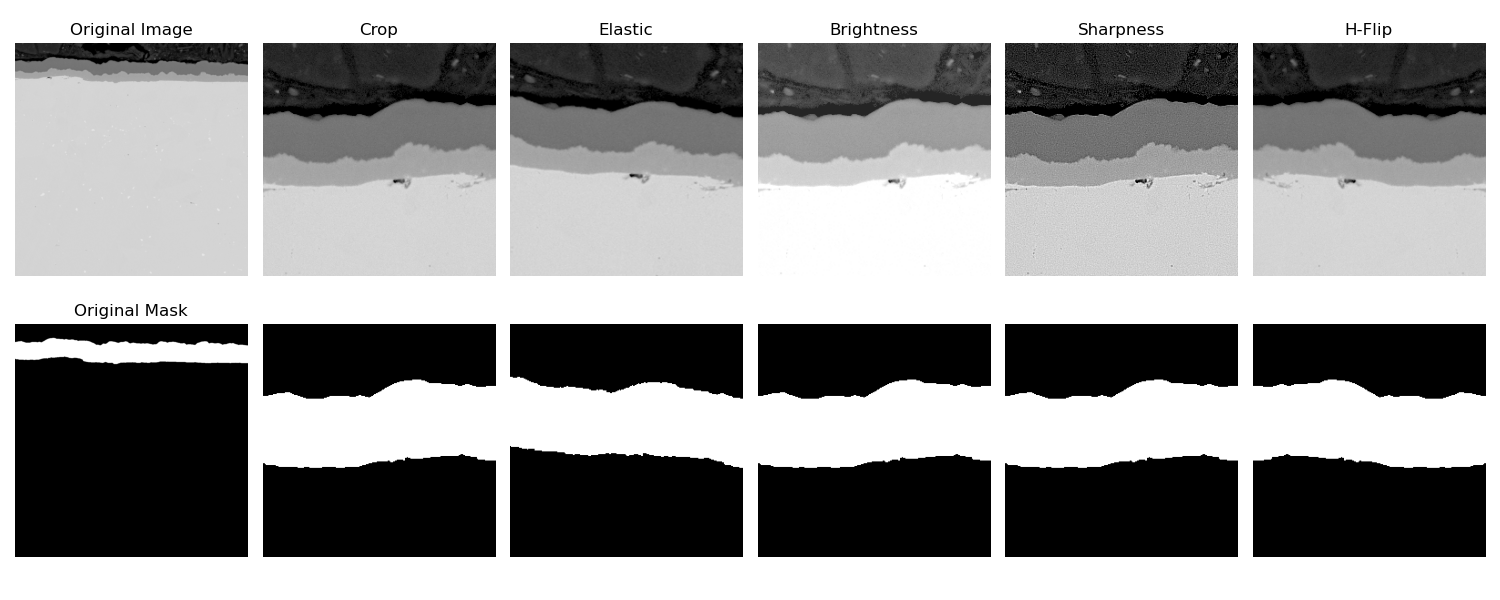
\includegraphics[width=1\linewidth]{PICTURES/augumentation.png}
\caption{Illustration of various augmentation techniques applied to the dataset.}
\label{fig:augmentation}
\end{figure}

\subsection{Technical Details}
The \texttt{segmentation\_models} library \cite{Iakubovskii:2019} was used for the U-Net implementation. Documentation for this implementation can be found \href{https://smp.readthedocs.io/en/latest/models.html#id21}{here} \cite{Iakubovskii_2019}. After initializing the training functions and other helper functions, hyperparameter tuning can begin. The main hyperparameters include depth, patch\_size, filters, and learning rates, all of which will be tested.

\subsection{Depth}
The depth of a U-Net is determined by the number of encoder and decoder blocks. This influences the model's ability to capture features within the input image. For instance, in Figure~\ref{fig:unet-architecture}, the depth is 5.

A deeper network (higher depth) can handle complex data with high variability, but may suffer from excessive downsampling and overfitting. In contrast, a shallower network may struggle to extract relevant features and differentiate between noise and useful information.

\subsection{Patch Size}
Patch size plays a crucial role in how well the model learns different features from the image.

Smaller patches allow the model to focus on fine details but might miss the broader context, making it harder to understand relationships between different parts of the image.

Larger patches capture more context and larger structures, but may lose fine details.

To ensure that the region of interest, specifically the coating layer, is always included, the images are cropped in a way that retains this key feature.

\subsection{Filters}
The filters parameter determines the number of filters used in each encoder and decoder layer, which affects the number of feature maps generated by the model. In the code, the number of filters in the decoder is calculated as follows:

\begin{verbatim}
decoder_channels = [filters * 2**i for i in range(depth, 0, -1)]
\end{verbatim}

This calculation, inspired by the original U-Net architecture, doubles the number of filters at each downsampling step \cite{2018arXiv180906839B}. For example, with \texttt{filters = 8} and \texttt{depth = 3}, the number of filters would be:  
\\\textbf{Encoder:} 8, 16, 32 \\
\textbf{Decoder:} 32, 16, 8

Using more filters allows the model to learn more complex patterns. However, it can also increase the risk of overfitting when there is insufficient training data. On the other hand, using fewer filters might prevent the model from capturing important features, reducing its performance.
\newpage
\subsection{Hyperparameter values}\label{sec:1.2.8}

In this project, all combinations of the following hyperparameters were tested:

\begin{itemize}
    \item \textbf{Patch size:} 128, 256
    \item \textbf{Depth:} 3, 4, 5
    \item \textbf{Filters:} 8, 16, 32
\end{itemize}

\subsection{Learning Rate and Schedulers}\label{sec:1.2.9}

During training, the model's parameters are adjusted to find the optimal solution. The \textbf{Adam optimizer} \cite{kingma2017adammethodstochasticoptimization} is used for this purpose. Adam (Adaptive Moment Estimation) calculates adaptive learning rates for each parameter.

Since Adam adapts the learning rate, manually modifying it can have a small impact but still affect performance. The learning rate is chosen from a range between 0 and the set value.

\begin{itemize}
    \item \textbf{Linear Scheduler:} The learning rate starts at the set value and decays linearly. The \textbf{end factor} multiplies the learning rate to finish at \textbf{end factor * lr}.
    \item \textbf{Warmup Cosine Scheduler:} The learning rate starts at a predefined value and decreases over \texttt{T\_0} epochs, following a cosine annealing schedule. After reaching the minimum, the learning rate resets and begins from the previous value, restarting the cycle.
\end{itemize}

The following schedulers and values were tested:
\begin{itemize}
    \item \textbf{LR values}: 0.01, 0.001, 0.0001
    \item \textbf{Linear scheduler}: With end factors of 0.01 and 0.001
    \item \textbf{Warmup Cosine scheduler}: With \texttt{T\_0}$= 25$ and \texttt{T\_0}$= 50$
\end{itemize}

Figure~\ref{fig:LRS} shows the learning rate schedulers. On the left, the linear scheduler spans 200 epochs, starting at 0.01 and ending at 0.001. On the right, the warmup cosine scheduler starts at 0.01 and ends at 0.00, with a warmup phase during the first 50 epochs.

\begin{figure}[H]
    \centering
    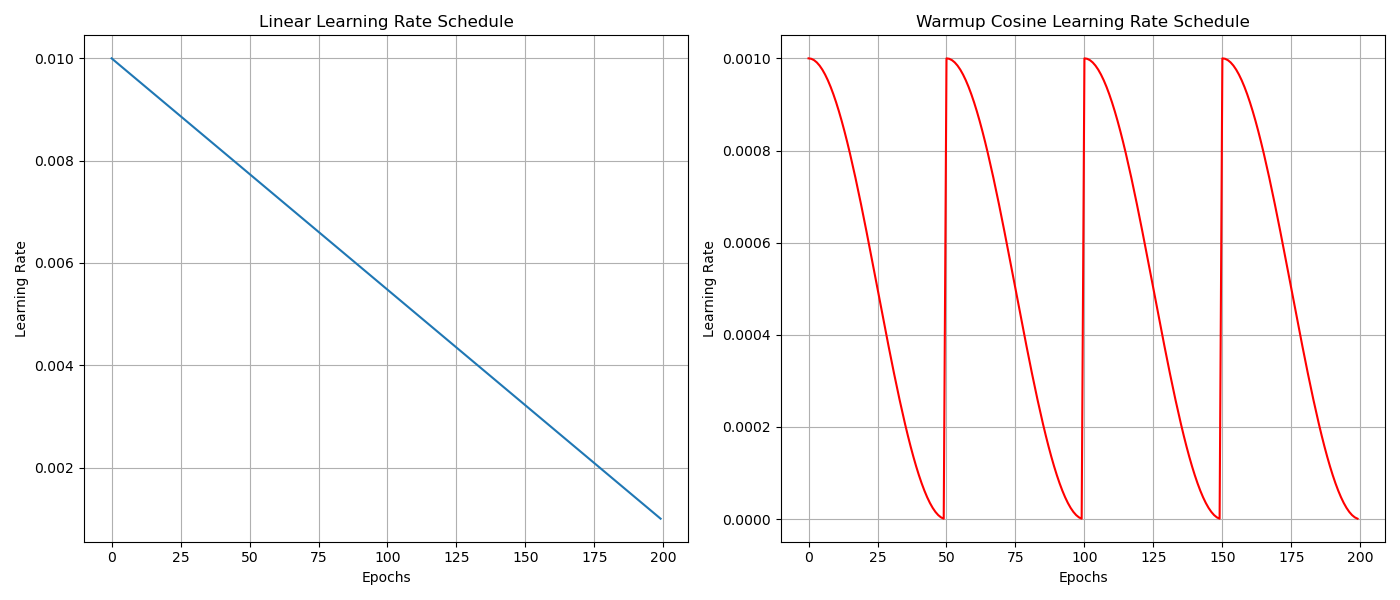
\includegraphics[width=0.9\linewidth]{PICTURES/LRS.png}
    \caption{Learning Rate Schedulers (LRS)}
    \label{fig:LRS}
\end{figure}
\subsection{Loss Function}

The loss function \( L(Y, \hat{Y}) \) is used to evaluate prediction errors. Since the model's performance on test data is assessed using the Intersection over Union (IoU) metric, IoU is also used as the loss function during training and validation.

The IoU is defined as:

\[
\text{IoU} = \frac{\text{intersection} + \text{smooth}}{\text{union} + \text{smooth}}
\]

Where:
\begin{itemize}
    \item The \( \text{intersection} \) is the number of pixels correctly predicted as the foreground (\(\text{True Positives}\)).
    \item The \( \text{union} \) consists of all pixels predicted or labeled as foreground. It equals the sum of \( \text{True Positives (TP)} \), \( \text{False Positives (FP)} \), and \( \text{False Negatives (FN)} \).
\end{itemize}

Thus, the IoU formula becomes:

\[
\text{IoU} = \frac{\text{TP} + \text{smooth}}{\text{TP} + \text{FP} + \text{FN} + \text{smooth}}
\]

The smoothing constant (\(\text{smooth} = 1\)) prevents division by zero. The loss function returns \( 1 - \text{IoU} \), ensuring that lower values indicate better model performance.

\subsection{Training}

After defining the key components, model training begins. The dataset is divided into 98 training images and 32 validation images. The training, validation, and testing labels come from the K-means refined dataset, with the validation set remaining fixed as a single batch.

During training, just the training data are shuffled each epoch to reduce the risk of overfitting. The shuffling function selects 32 random images for each batch. Training proceeds for either 200 or 150 epochs, with each epoch consisting of both training and validation phases.

\subsubsection{Training Phase}

In each epoch, the training dataset is shuffled, and three batches of 32 images are formed. The model predicts the binary mask for each batch and computes the training loss. Backpropagation adjusts the model's parameters using the optimizer based on the computed loss.

\subsubsection{Validation Phase}

At the end of each epoch, the validation set (a single batch) is evaluated using the loss function. The model's parameters are not updated during this phase. If the validation loss is lower than the previously recorded minimum, the model and its parameters are saved, and the minimum validation loss is updated.

\subsection{Optimization Strategy}

\begin{enumerate}
    \item Three optimization runs were performed to determine the optimal learning rate (LR) and learning rate scheduler. Details about the hyperparameters tested are provided in section \ref{sec:1.2.9}.
    \item The main optimization focused on the three key hyperparameters, using the best LR and LR scheduler from the initial optimization. The specific hyperparameters optimized are discussed in section \ref{sec:1.2.8}.
    \item After identifying the best hyperparameters, two additional runs were conducted. One used polygon labels, while the other used non-refined K-means labels.
\end{enumerate}
\subsection{Optimization results}

The optimization of the learning rate and learning rate schedulers is discussed first. The schedulers were tested with the hyperparameters \textbf{depth = 3}, \textbf{patch size = 128}, and \textbf{filters = 8}. These values were chosen as they offered the best computational efficiency among the tested ones. Initially, the warmup cosine scheduler was optimized. The contour plot below illustrates the relationship between \( T_0 \) and the learning rate. The optimal point occurs at \( T_0 = 50 \) and \( \text{lr} = 0.01 \), resulting in a minimum objective function value (IoU validation loss) of 0.03306.

\begin{figure}[H]
    \centering
    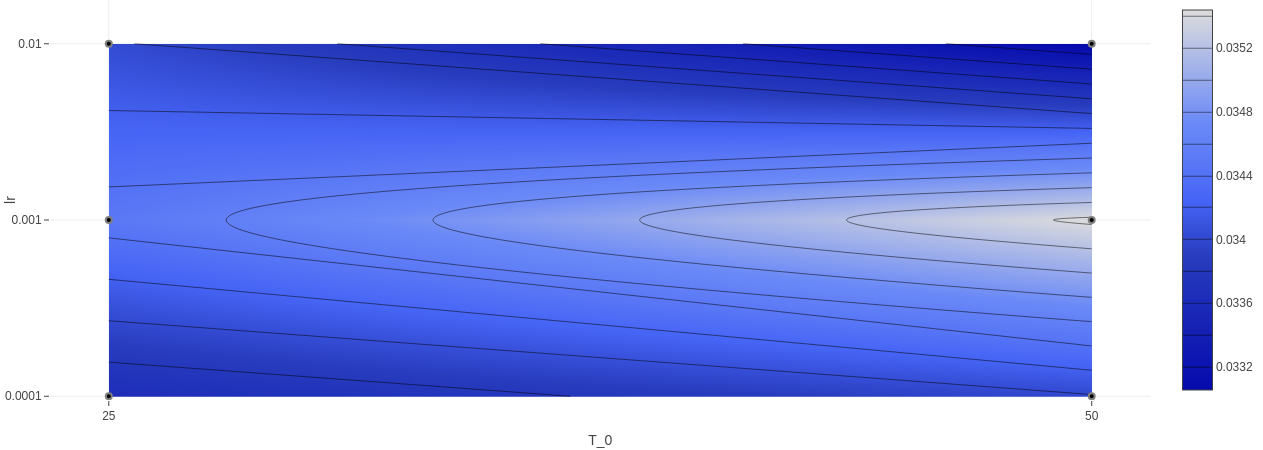
\includegraphics[width=0.75\linewidth]{PICTURES/cosine.png}
    \caption{Objective function contour: effect of \( T_0 \) and Learning Rate}
    \label{fig:cosine_contour}
\end{figure}

The best results for different learning rate schedulers are summarized in Table \ref{tab:scheduler_results}. The linear scheduler achieved the lowest objective function value of 0.03075 with a learning rate of 0.001 and an end factor of 0.001. The optimization without a scheduler resulted in a minimum objective function value of 0.03133 at a learning rate of 0.01.

\begin{table}[H]
    \centering
    \begin{tabular}{lccc}
        \toprule
        Schedule & Learning Rate (lr) & End Factor / \( T_0 \) & Val Loss \\
        \midrule
        Warmup Cosine & 0.01 & 50 & 0.03306 \\
        Linear & 0.001 & 0.001 & 0.03075 \\
        None & 0.01 & --- & 0.03133 \\
        \bottomrule
    \end{tabular}
    \caption{Best results for different Learning Rate Schedulers.}
    \label{tab:scheduler_results}
\end{table}

\newpage
Next, the main optimization was conducted using the linear scheduler and the best values from the previous step. The hyperparameters discussed in section \ref{sec:1.2.8} were optimized, resulting in 18 combinations (2 * 3 * 3 = 18). The complete results are shown in Table \ref{tab:main_results}, with the best result found at index 9.

\begin{table}[H]
\centering
\renewcommand{\arraystretch}{1}
\begin{tabular}{|c|c|c|c|c|}
\hline
\textbf{Idx} & \textbf{Val Loss} & \textbf{Depth} & \textbf{Filters} & \textbf{Patch Size} \\
\hline
0  & 0.03315 & 5  & 8   & 256 \\
1  & 0.03902 & 5  & 8   & 128 \\
2  & 0.03204 & 3  & 8   & 256 \\
3  & 0.03365 & 5  & 16  & 256 \\
4  & 0.02999 & 5  & 32  & 256 \\
5  & 0.03192 & 4  & 8   & 128 \\
6  & 0.03047 & 4  & 16  & 256 \\
7  & 0.03307 & 3  & 8   & 128 \\
8  & 0.03406 & 4  & 8   & 256 \\
\textbf{9}  & \textbf{0.02892} & \textbf{5}  & \textbf{16}  & \textbf{128} \\
10 & 0.03502 & 3  & 32  & 128 \\
11 & 0.03136 & 5  & 32  & 128 \\
12 & 0.03001 & 4  & 16  & 128 \\
13 & 0.02910 & 4  & 32  & 128 \\
14 & 0.03108 & 3  & 16  & 256 \\
15 & 0.03036 & 4  & 32  & 256 \\
16 & 0.03271 & 3  & 32  & 256 \\
17 & 0.03289 & 3  & 16  & 128 \\
\hline
\end{tabular}
\caption{Validation loss values with Depth, Filters, and Patch Size}
\label{tab:main_results}
\end{table}

Figure \ref{fig:validation_loss} presents the validation loss values over 150 epochs. Initially, both curves decrease rapidly, then oscillate around similar values, suggesting that the parameters no longer change significantly. The yellow line represents the best optimization, while the purple line represents the second-best optimization. From epoch 100 onward, the results stabilize. The optimization at index 9 provides the best performance. This model will be evaluated on the test dataset and implemented into the researcher's workflow.

\begin{figure}[H]
    \centering
    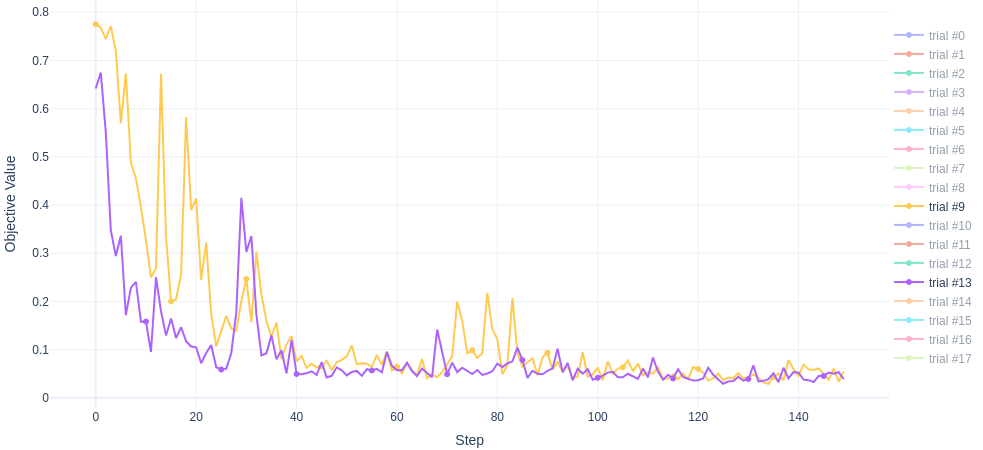
\includegraphics[width=0.75\linewidth]{PICTURES/lossFuncMain.png}
    \caption{Validation loss over 150 epochs}
    \label{fig:validation_loss}
\end{figure}

Additionally, Figure \ref{fig:Hyperparameter-Importance} shows the feature importances, indicating that patch size has the greatest impact on the results. This insight can be used in future work.

\begin{figure}[H]
    \centering
    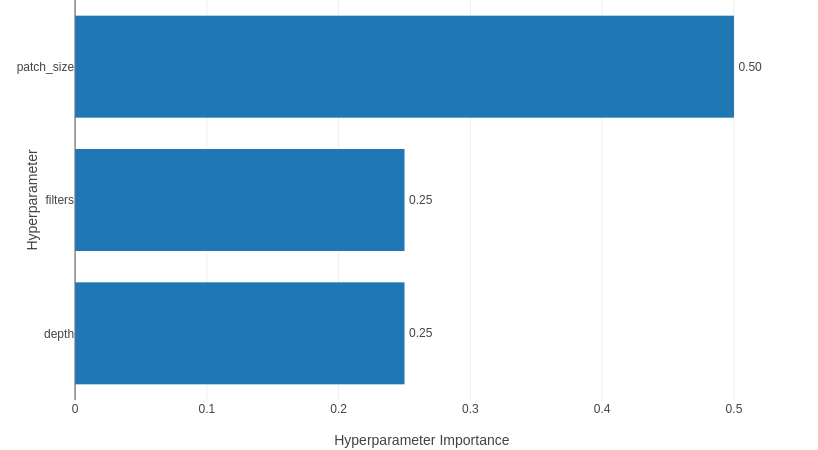
\includegraphics[width=0.75\linewidth]{PICTURES/importnace.png}
    \caption{Hyperparameter importance}
    \label{fig:Hyperparameter-Importance}
\end{figure}

The final two runs were conducted using the best hyperparameters, but with datasets that included labels generated by polygons and K-means clustering. The corresponding validation loss values are presented in Table \ref{tab:val_loss_values}.

\begin{table}[ht]
\centering
\renewcommand{\arraystretch}{1}
\begin{tabular}{|c|c|c|c|}
\hline
\textbf{Metric} & \textbf{K-means Refined} & \textbf{K-means} & \textbf{Polygon} \\
\hline
Validation Loss & 0.02892 & 0.03118 & 0.09698 \\
\hline
\end{tabular}
\caption{Validation loss values for different labeling methods}
\label{tab:val_loss_values}
\end{table}

Since both validation sets use labels from their respective training sets, these values may not be fully reliable. It is better to assess the model’s performance on unseen images using test labels generated from K-means refined clustering. Although the K-means and polygon labels are not intended for use in the final workflow, evaluating their performance on real test data could still provide useful insights.

\subsection{Evaluation on Test Data}

Two primary evaluation metrics were used:

\begin{itemize}
    \item \textbf{Mean IoU}: The intersection over union (IoU) is calculated and averaged across all test data.
    \item \textbf{Min IoU}: The minimum IoU value is used to assess the worst-case scenario.
\end{itemize}

The evaluation results are presented in Table \ref{tab:test_results}:

\begin{table}[ht]
\centering
\renewcommand{\arraystretch}{1.2}
\begin{tabular}{|c|c|c|c|}
\hline
\textbf{Metric} & \textbf{K-means Refined} & \textbf{K-means} & \textbf{Polygon} \\
\hline
Mean IoU & 0.95473 & 0.83111 & 0.92177 \\
Min IoU & 0.83872 & 0.17518 & 0.78456 \\
\hline
\end{tabular}
\caption{Evaluation Results on Test Data}
\label{tab:test_results}
\end{table}

The results reveal some key patterns. Although the "polygon" model was trained on validation data with polygon labels, it still performed well. This suggests that polygon labels could be used instead of K-means refined labels when applying the model to other parts of the images, such as various oxidation layers. They can also be used when retraining the model once more data is gathered. In such cases, K-means refinement may not be necessary, as polygon labels can be efficiently generated with a single script. On the other hand, the K-means labels without refinement performed poorly. This likely occurred because the model struggled to differentiate between oxidation and coating layers, which were not well-separated in the training data. In contrast, the K-means refined labels provided the best results on unseen data.

\newpage

\begin{figure}[H]
    \centering
    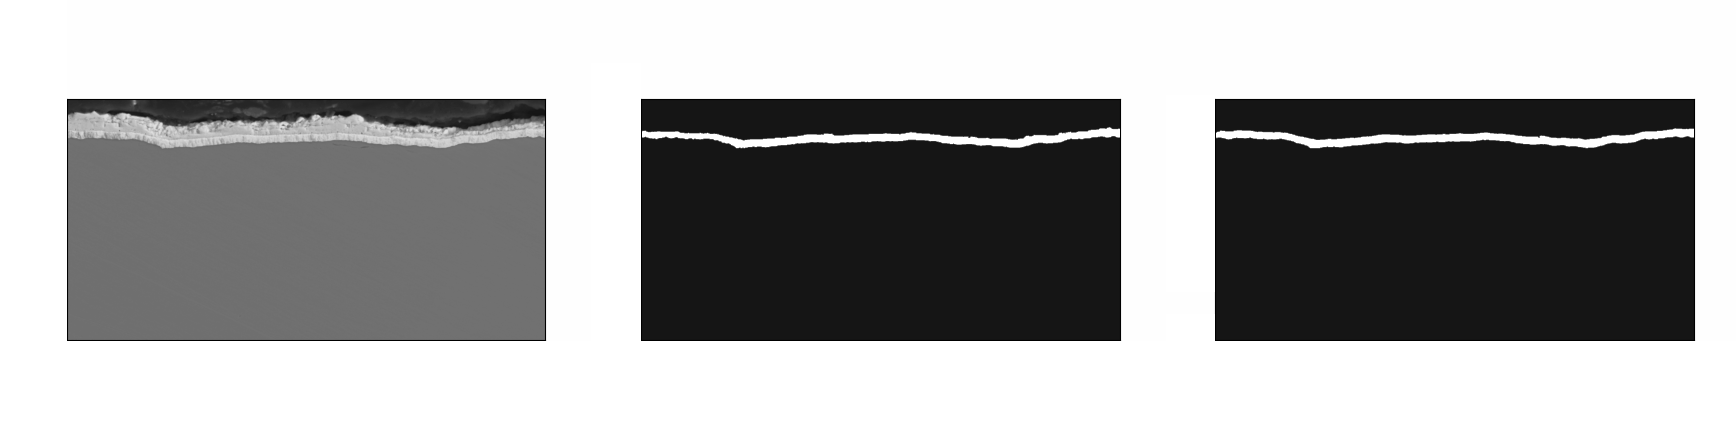
\includegraphics[width=1\linewidth]{PICTURES/refined_188_5_128_16_9.png}
    \caption{Original image, ground truth, prediction (K-means refined model)}
    \label{fig:refined_188_5_128_16_9}
\end{figure}

\begin{figure}[H]
    \centering
    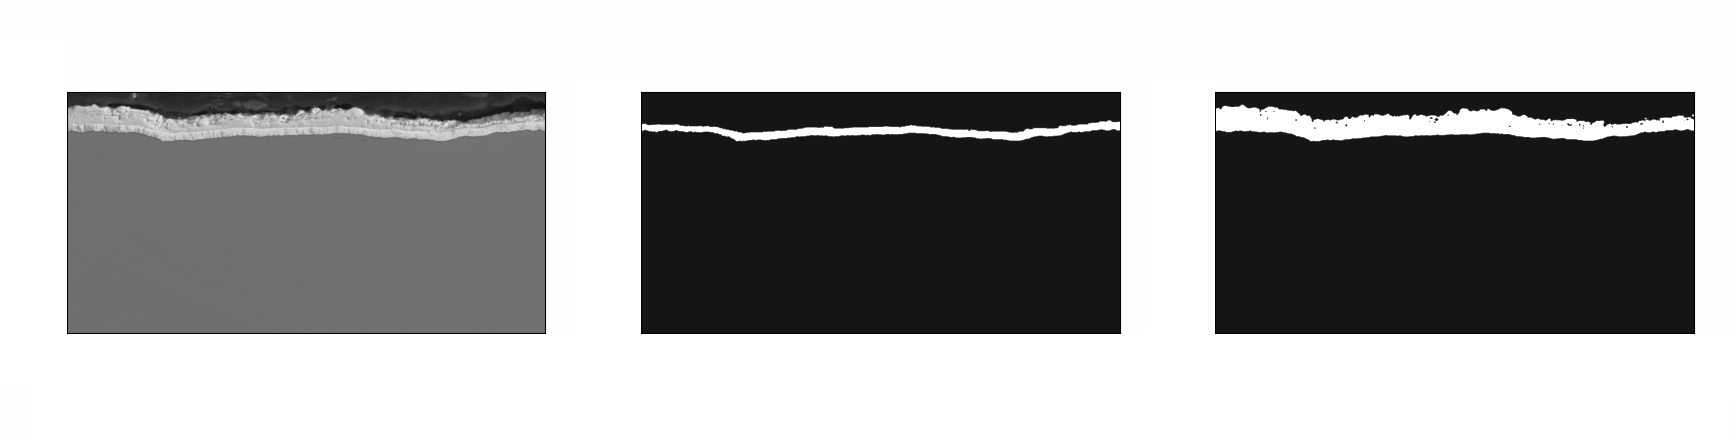
\includegraphics[width=1\linewidth]{PICTURES/kmeans_188_5_128_16_0.png}
    \caption{Original image, ground truth, prediction (K-means model)}
    \label{fig:kmeans_188_5_128_16_0}
\end{figure}

\begin{figure}[H]
    \centering
    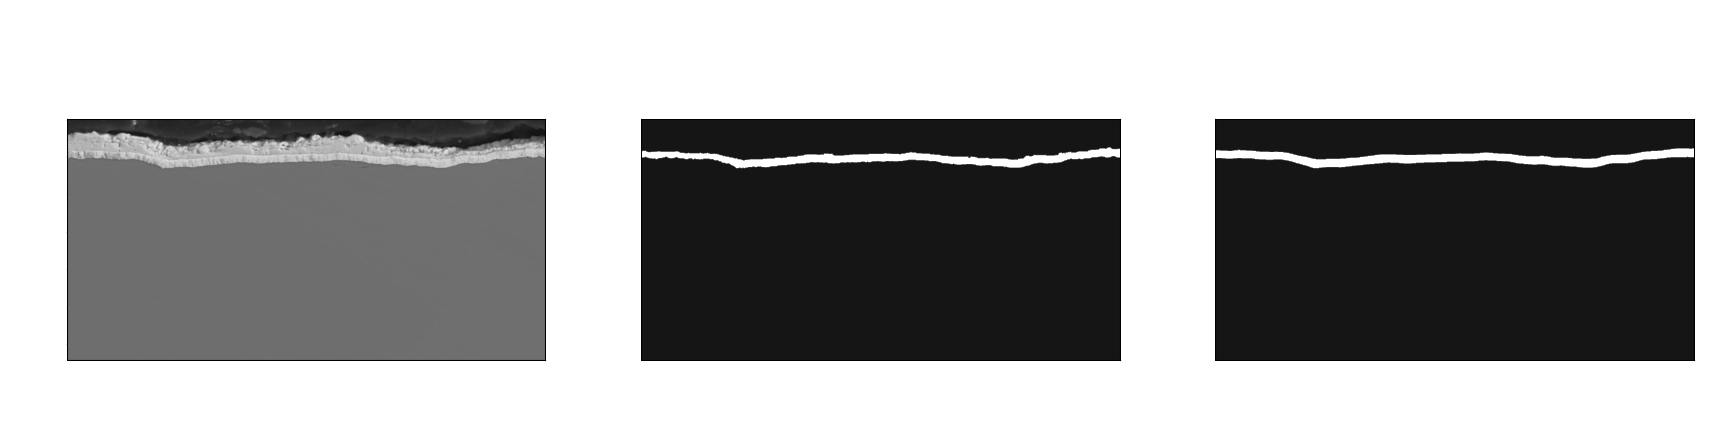
\includegraphics[width=1\linewidth]{PICTURES/polygon_188_5_128_16_0.png}
    \caption{Original image, ground truth, prediction (polygon model)}
    \label{fig:polygon_188_5_128_16_0}
\end{figure}

Figure \ref{fig:kmeans_188_5_128_16_0} illustrates that the model struggles to recognize the oxidation and coating layers, resulting in poor performance. In contrast, Figures \ref{fig:polygon_188_5_128_16_0} and \ref{fig:refined_188_5_128_16_9} demonstrate that the models can accurately predict coating layers, even though the images are complex and distinguishing between the layers is difficult.

\section{Integration of the Model}

After training the model, it was crucial to integrate it smoothly into the existing workflow to avoid requiring the researcher to learn new software. The model was integrated into the Fiji software, which was already in use, instead of creating a new application.

The first step involved adding a new button to the Fiji interface, as shown in Figure~\ref{fig:enter-label-2}. Pressing this button triggers a Python script from the `StartupMacro`, with the path to the image being analyzed passed as an input argument. The script, stored in the Fiji application folder along with the macros and model parameters, loads the image and crops the lower part to remove irrelevant information. It then predicts a binary mask, processes it, and extracts the ten most relevant lines.

By default, another set of ten lines is added beneath the first set. The resulting data, containing the twenty lines, are saved in a zip folder. The path to this zip folder is then returned, and Fiji opens the folder to display the predicted lines to the researcher. If the researcher is dissatisfied with the predictions, they can modify the lines as needed.

\begin{figure}[ht]
    \centering
    \begin{subfigure}{0.45\textwidth}
        \centering
        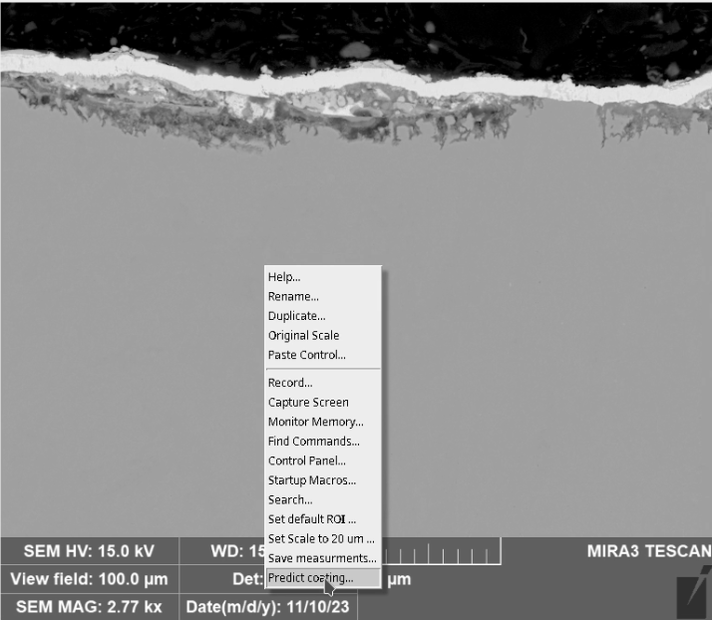
\includegraphics[width=\linewidth]{PICTURES/fiji/frame-002.png}
        \caption{Menu with \textit{Predict coating...} button}
        \label{fig:enter-label-2}
    \end{subfigure}
    \begin{subfigure}{0.45\textwidth}
        \centering
        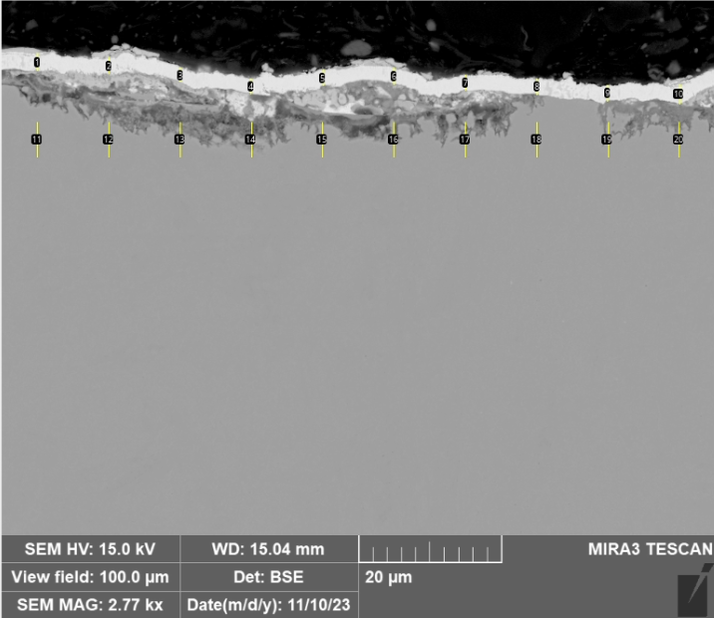
\includegraphics[width=\linewidth]{PICTURES/fiji/frame-003.png}
        \caption{Predicted lines}
        \label{fig:enter-label-3}
    \end{subfigure}
    \caption{Example workflow in Fiji}
    \label{fig:two-masks}
\end{figure}
\newpage
\section{Results - Time Experiment}

Following the model integration and the update to the Fiji setup, a time measurement study was conducted to assess time savings. Eight images were selected from four batches, with two images chosen from each batch. The experiment was designed as follows:

The first image in the set is measured manually, while the second is analyzed using the prediction model. In the first image from the first set, only the predefined default lines were used, simulating the first image in each batch where the researcher does not have lines similar to the coating. The first image from the second set used predefined lines from another image in the same batch. Since the images in each batch are similar, the researcher typically spends less time adjusting these lines. The third set followed the same approach as the second, but with an image where the model did not predict all the lines correctly. The fourth set included a challenging image with complex oxidation, where the model's predictions were less accurate, though the same approach as the second set was used on the first image.

The "Model" column in Table~\ref{tab:time-measurements} indicates whether the model was used for line prediction. The model was not used for the first image in each set but was used for the second image.

The "Predict" column shows the time from pressing the "Predict coating" button until the predicted lines were displayed, which took approximately 14 seconds, depending on the computer hardware. 

The "Measure" column represents the total time from starting the prediction (or manual measurement with predefined lines) to when the researcher finished editing. 

The "Add\_Excel" column reflects the time the researcher took from the start until adding the measurements to the Excel file. When using the model, the researcher worked with an updated version of Fiji, which included the improvements described in \textit{Fiji adjustments} (\ref{sec:1.2.2}). Consequently, Fiji, with the model, was also able to export to Excel faster.


\begin{table}[H]
\centering
\begin{tabular}{|l|l|l|l|l|}
\hline
\textbf{Type}           & \textbf{Model} & \textbf{Predict} & \textbf{Measure} & \textbf{Add\_Excel} \\ \hline
First Batch             & N             & /                & 01:12.00         & 01:30.00         \\ \hline
First Batch             & Y             & 00:14.00         & 00:28.00         & 00:38.44         \\ \hline
Normal                  & N             & /                & 00:57.32         & 01:26.00         \\ \hline
Normal                  & Y             & 00:14.00         & 00:25.20         & 00:38.34         \\ \hline
Model Wrong             & N             & /                & 01:09.00         & 01:32.00         \\ \hline
Model Wrong             & Y             & 00:14.00         & 00:57.32         & 01:10.00         \\ \hline
Hard Oxidation          & N             & /                & 01:05.00         & 01:26.00         \\ \hline
Hard Oxidation          & Y             & 00:14.00         & 00:45.24         & 00:59.00         \\ \hline
\end{tabular}
\caption{Time measurement results for four sets of images. All times are in min:s:ms.}
\label{tab:time-measurements}
\end{table}
\subsection{Time per one batch}

A theoretical batch of 30 images was considered for this experiment. It was assumed that the first image in the batch would take the longest to process, as is explained in \ref{sec:ManualProc}. Additionally, two images were expected to experience significant model errors, while two others presented challenging oxidation conditions. The time spent on measurement with the model was approximated as:

\[
\text{Time with model} = 28 + (25 \times 25) + (57 \times 2) + (45 \times 2) = 857 \text{ seconds} = \frac{857}{60} \approx 14.28 \text{ minutes}.
\]

The results of the time calculations are summarized in Table \ref{tab:time_comparison}.

\begin{table}[H]
    \centering
    \renewcommand{\arraystretch}{1}
    \begin{tabular}{|c|c|c|}
        \hline
        \textbf{Scenario} & \textbf{Time (seconds)} & \textbf{Time (minutes)} \\
        \hline
        Model - Measure & 857 & $\frac{857}{60} \approx 14.28$ \\
        \hline
        Manual - Measure & 1765 & $\frac{1765}{60} \approx 29.42$ \\
        \hline
        Model - Total & 2596 & $\frac{2596}{60} \approx 43.27$ \\
        \hline
        Manual - Total & 1246 & $\frac{1246}{60} \approx 20.77$ \\
        \hline
    \end{tabular}
    \caption{Comparison of time taken in different scenarios}
    \label{tab:time_comparison}
\end{table}

The percentage reductions in time are presented in Table \ref{tab:percentage_reduction}:

\begin{table}[H]
    \centering
    \renewcommand{\arraystretch}{1}
    \begin{tabular}{|c|c|}
        \hline
        \textbf{Scenario} & \textbf{Percentage reduction} \\
        \hline
        Reduction in measurement time & $\frac{29.42 - 14.28}{29.42} \times 100 \approx 51.5\%$ \\
        \hline
        Reduction in total time & $\frac{43.27 - 20.77}{43.27} \times 100 \approx 52.0\%$ \\
        \hline
    \end{tabular}
    \caption{Percentage reduction in measurement and total time}
    \label{tab:percentage_reduction}
\end{table}

Thus, using the model results in significantly faster processing times for measurement and saving results. Although these measurements are approximations, the results clearly demonstrate that the model improves the speed of the process.

\section{Results - Precision}

After the model was integrated into the workflow, data were collected from the research process. A total of 90 images were analyzed using the model. For each image, two folders were generated: one containing the predicted lines and another for the lines that could be manually adjusted by the researcher. The results from three separate batches are summarized below.

The first and second batches showed high accuracy, requiring minimal manual adjustments. However, the third batch exhibited reduced performance. This decline was attributed to the introduction of different types of layers. Notably, the model also detected the white oxidation layer above the coating layer, as shown in Figure~\ref{fig:ox}. This layer is visually similar to other structural layers, as seen in Figure~\ref{fig:three-images} (right image).

\begin{figure}[H]
    \centering
    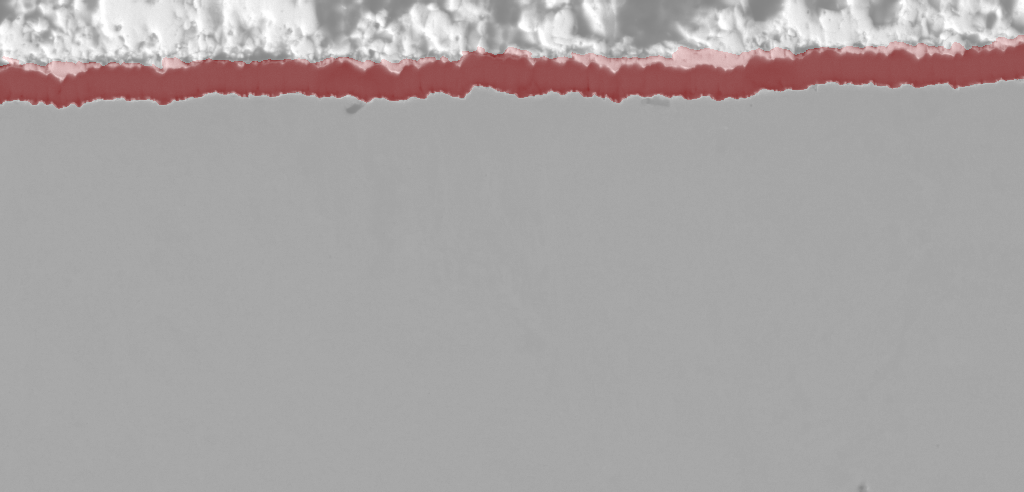
\includegraphics[width=0.5\linewidth]{PICTURES/aa.png}
    \caption{Image from the third batch, highlighting a poor prediction.}
    \label{fig:ox}
\end{figure}

These results suggest that the model performs well overall, requiring only minor adjustments in most of the cases. However, the findings also highlight the need to obtain a bigger dataset. The current dataset is still relatively small. These new data can be incorporated into the dataset using polygon labels, which can be efficiently created using automated scripts. After this, the model can be re-trained to make it more robust. This will create a feedback loop where labels can be generated faster, leading to a larger dataset, which in turn, after re-training, improves overall precision and results in time savings.

The precision of the model's predictions was evaluated by counting the number of points that required manual adjustment after the predictions were made. Table~\ref{tab:results} presents the summary statistics for the three analyzed batches.

\begin{table}[H]
    \centering
    \begin{tabular}{lcc}
        \toprule
        \textbf{Batch} & \textbf{Mean difference (pixel)}  & \textbf{Unchanged Points (\%)} \\
        \midrule
        1 & 1.11  & 93.3\% (560/600) \\
        2 & 0.57  & 97.3\% (584/600) \\
        3 & 5.58  & 22.7\% (136/600) \\
        \bottomrule
    \end{tabular}
    \caption{Analysis of model predictions across three batches.}
    \label{tab:results}

\end{table}

As shown in Table~\ref{tab:results}, the first two batches display a high percentage of unchanged points, indicating that the model's predictions are highly accurate. In contrast, the third batch shows a significantly higher mean difference and a lower percentage of unchanged points. This highlights the need for additional data to improve the model's performance.







\begin{comment}
\subsection{Evaluation}
To properly evaluate each model so they can be compared evaluation metrics need to be defined.  
\subsection{IoU}
IoU quantifies the overlap between the predicted mask and the actual layer, revealing how well the model captures the layer.  Equation 1 shows the mathematical formula for IoU. From the library torchmetrics, JaccardIndex can be imported. That is analogous to IoU. 
\subsection{    Average Start-End Differences }
This metric measures the average absolute difference between the start and end points of detected lines compared to researcher-marked lines (ground truth). Each image can have a maximum of 10 lines.  

If a researcher hasn't marked a line (resulting in NaN), the difference for both starts and endpoints is recorded as NaN in the results. 
\subsection{    Average Length DifferenceS }
This is the average length difference of the predicted 10 lines per mask and the ground truth. It penalizes the nan values the same way as 3.2. 
\subsection{    Mean Squared Error (MSE) of Differences }
The Mean Squared Error (MSE) of differences builds upon metrics 3.2 and 3.3. Unlike the mean absolute difference, MSE squares the errors before averaging them. This approach assigns greater weight to larger errors, making it more sensitive to outliers. Since large errors are particularly problematic in this project, MSE is a well-suited metric for evaluating the accuracy of line detections. 

\section{Connection to Fiji}
To integrate the trained model into Fiji, an existing startup macro was utilized. This macro opens and executes a Python script, which serves as an Application Programming Interface (API). The Python script begins by taking an image and the number of lines to be detected as input. It then uses a pre-trained model, represented by a .pth file, to predict a mask for the image. 

Following the prediction, the mask undergoes a three-stage post-processing procedure to eliminate noise and incorrect predictions. First, all white clusters within the predicted mask are converted into an array. The script then identifies clusters that touch both the left and right borders of the image—since such clusters are most common. If no such clusters are found, the script looks for the largest cluster that touches either the left or right borders. This step is particularly useful when intense oxidation occurs in the middle of the image. If neither of these criteria is met, the script selects the largest cluster available. 

Here are some images to demonstrate various types of postprocessing 

Once the mask is processed, it is sent to another function that generates the regions of interest (ROIs) that researchers need. This function uses a library to generate lines based on the first and last occurrences of white pixels in the mask, aligned with the y-axis at specific x-coordinates predefined by the researcher. If no lines are found, default lines are generated. Additionally, a second set of lines is produced below the first 10 predicted lines on default places. This second set is important because researchers are also measuring oxidation on minority samples when it occurs. 

The generated lines are then saved into a zip file, and the path to this zip file is communicated back to the Fiji application. The Fiji application then automatically opens the zip file, presenting the lines to the user. This entire process is hidden from the user; they only need to click on the model button and wait for a short duration, depending on the type of computer, after which the lines will appear. researchers can inspect these lines and, if necessary, edit them, just as they were able to do before. 
\end{comment}




\chapter{Conclusion}

This thesis successfully addresses the challenge of automating a time-consuming manual process in the nuclear industry. Researchers are often required to perform repetitive, labor-intensive measurements. The primary goal was to develop a solution that integrates seamlessly into the researcher’s workflow without causing disruptions. The thesis focused on a specific category of coating-layer images with relatively homogeneous properties, in contrast to other images in the dataset. It was shown that segmentation of more complex, heterogeneous images is a viable direction for future work.

Three approaches were evaluated. First, the classical K-means algorithm was found to be computationally efficient, but it lacked universal applicability due to the variability of coating layers. This made it unsuitable for a streamlined workflow without extensive post-processing. Second, the Segment Anything Model (SAM) was considered, but hardware limitations made it infeasible for the given problem. Finally, Convolutional Neural Networks (CNNs) were explored. This solution required labeled data. Three types of labels were developed. The model was trained on the most precise set, but it was found that even the least manually intensive labels were effective for training, despite being less accurate. This insight suggests that efficient model retraining is also possible with this kind of labels and that the model could be adapted to handle more complex images in the future.

The optimization and testing of the model were thoroughly discussed, with results measured using the Intersection over Union (IoU) metric. The model achieved a mean IoU of 95.47\%, demonstrating its high accuracy in segmenting coating layers.

After integrating the model into the researcher’s workflow, the practical impact was clear. The time required for measurement tasks was reduced by half. For images similar to the training dataset, over 90\% of predicted measurements required no further manual adjustments. However, for images from batches with significantly different characteristics, performance declined, highlighting the need for further re-training.

With the code infrastructure in place, future improvements can focus on streamlining the training process and enhancing prediction accuracy. The current model was trained on fewer than 100 images from a limited number of batches, which is insufficient for creating a fully robust model. Nevertheless, even when incorrect, the model's average deviation was approximately five pixels, resulting in substantial time savings. This efficiency will accelerate the generation of additional labeled data, creating a feedback loop for continuous improvement. The iterative workflow is illustrated in figure~\ref{fig:workflow-diagram}.

\begin{figure}[H]
    \centering
    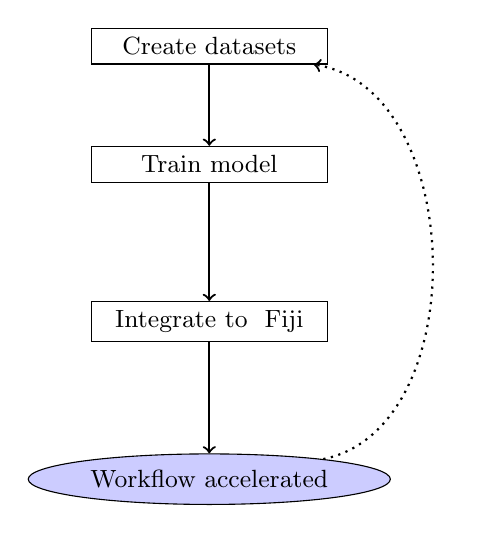
\begin{tikzpicture}[node distance=1.5cm, every node/.style={align=center, font=\small}]

        \node[rectangle, draw, minimum width=3cm] (dataset) {Create datasets};
        \node[rectangle, draw, minimum width=3cm, below of=dataset, yshift=0cm] (train) {Train model};
        \node[rectangle, draw, minimum width=3cm, below of=train, yshift=-0.5cm] (integration) {Integrate to \ Fiji};
        \node[ellipse, draw, fill=blue!20, minimum width=3cm, below of=integration, yshift=-0.5cm] (result) {Workflow accelerated};

        % Arrows
        \draw[->, thick] (dataset) -- (train);
        \draw[->, thick] (train) -- (integration);
        \draw[->, thick] (integration) -- (result);
        \draw[->, thick, dotted] (result) to[bend right=80] (dataset);
    \end{tikzpicture}
    \caption{Workflow of model integration and performance improvement.}
    \label{fig:workflow-diagram}
\end{figure}

In conclusion, this thesis automates a portion of the researcher’s measurement process and establishes a pipeline for continuous model retraining and improvement. It also demonstrates that polygon masks, generated directly from researcher annotations, are sufficient for training segmentation models. These results suggest that similar models can be developed for other types of images within the researcher’s domain. The improvements brought by this work will lead to time savings and improved efficiency. This work highlights the practical impact of deep learning in automating image analysis tasks in the nuclear industry.

\chapter{Appendix}

The complete implementation of this thesis, including preprocessing, label generation, model training, and evaluation scripts, is available at [GitHub Repository Link (will be added in future when it has documentation, proper README,...)].

This project benefited from various open-source libraries that facilitated image processing, deep learning model training, and evaluation. A detailed list of dependencies and libraries used can be found in the repository’s requirements.txt file.

Additionally, this text was refined and grammar-checked using ChatGPT \cite{chatgpt2025}, and Grammarly \cite{grammarly2025}.


\bibliographystyle{plain}
\bibliography{CNN}


\newpage
\listoffigures
\newpage

\listoftables
\newpage

\chapter*{List of Abbreviations}
\begin{itemize}
    \item \textbf{TP} - True Positive
    \item \textbf{TN} - True Negative
    \item \textbf{FP} - False Positive
    \item \textbf{FN} - False Negative
    \item \textbf{CNN} - Convolutional Neural Network
    \item \textbf{LR} - Learning Rate
    \item \textbf{LRS} - Learning Rate Scheduler
    \item \textbf{SEM} - Scanning electron microscope
    \item \textbf{IoU} - Intersection over union
    %\item \textbf{ROI} - Region of interest (here, measurement lines)
    \item \textbf{SAM} - Segment Anything Model
\end{itemize}




\end{document}
